\section{Introduction}
In the era of information overload, recommender systems play a pivotal role in various online services, which aim to match user interests with resource items~\cite{sarwar2001item}.
Classic recommendation methods, \eg matrix factorization~\cite{koren2015advances}, mainly model users' preference towards items using historical user-item interaction records. Nowadays, various kinds of auxiliary data become increasingly available in online services. Many methods further propose to leverage these context information for improving recommendation performance~\cite{ronen2016recommendations,adomavicius2015context}.
Due to the heterogeneity and complexity of auxiliary data, it is still challenging to effectively utilize such context information in recommender systems.


%With the rapid growth of Web techniques, various kinds of auxiliary data become available in recommender systems. Although auxiliary data is likely to contain useful information for recommendation~\cite{}, it is difficult  to effectively utilize these heterogeneous and complex information in recommender systems.

%Recommender systems mainly aim to model users's preference towards items based on the historical user-item interaction records (\eg user-item rating matrix), known as collaborative filtering~\cite{he2016fast}. In this setting, matrix factorization (MF) remains as one of the most popular collaborative filtering techniques, which simply models the interaction between users and items as the inner product of their latent factors. Despite the effectiveness of MF for recommendation, it may be not sufficient to capture the complex structure of user interaction data via the simple multiplication of latent features linearly.

As a promising direction, \emph{heterogeneous information network} (HIN), consisting of multiple types of nodes and links, has been proposed as a general information modeling method~\cite{sun2011pathsim,shi2017survey}.
Since HIN is flexible to characterize various kinds of heterogenous data, it has been adopted
  in recommender systems to model rich auxiliary data~\cite{zhao2017meta,yu2014personalized}.
In particular,  \emph{meta-path},  a relation sequence connecting object pairs in HIN, is widely used to extract structural features that capture relevant  semantics  for recommendation~\cite{sun2011pathsim}.
We present an example for movie recommendation characterized by HIN in Fig.~\ref{fig-framework-intro}(a).
Roughly speaking, existing HIN based recommendation methods can be categorized into two types.
The first type leverages path based semantic relatedness over HIN as \emph{direct features} for recommendation relevance~\cite{feng2012incorporating,yu2014personalized,shi2015semantic}.  %These methods usually utilize meta-paths to extract or characterize structural features of object pairs, which is mainly used for similarity measurement.
As a comparison, the second type performs some transformation  on path based similarities (\eg matrix factorization on the path based similarity matrix) for learning effective \emph{transformed features}, which are subsequently used to enhance original user or item representations in the recommendation methods~\cite{yu2014personalized,zhao2017meta}.
These two types of methods both extract meta-path based features for improving the characterization of two-way user-item interaction, as illustrated in Fig.~\ref{fig-framework-intro}(b).
%The two types of methods correspond to the full line and dot dash line respectively in Fig.~\ref{fig-framework-intro}(b).

%Existing methods Recently, a number of methods have been proposed to exploit the rich relations in HIN, which can be roughly categorized  into two types. (1) One type of methods learn the latent factors (or embeddings) of users and items for recommendation (see the full line in Figure 1(b))\cite{yu2013collaborative,luo2014hete,shi2016integrating}. These methods usually factorize a matrix of users and items, which is the interaction matrix (e.g., rating matrix) or relation matrix extracted from meta paths, under the matrix factorization framework. Recently, some deep neural network are also been employed to learn refined latent factors \cite{he2017neural,tay2018latent}. (2) The other type of methods leverage path based semantic relatedness between users and items over HINs for recommendation (see the dot dash line in Figure 1(b))\cite{feng2012incorporating,yu2013collaborative,yu2014personalized,shi2015semantic,shi2016integrating}.  These methods usually utilize meta paths to extract or measure structure features of object pairs (e.g., similarity measure), which can also been seen as a kind of embedding information. With the surge of network embedding, path based node embedding in HIN can also been used for recommendation \cite{dong2017meta-path2vec,fu2017hin2vec}.


%Under the HIN-based representation, the recommendation problem can be considered as a similarity search task over the HIN~\cite{sun2011pathsim}.
%Such a recommendation setting is called as \emph{HIN-based recommendation}~\cite{yu2013collaborative}.
%HIN-based recommendation has received much attention in the literature~\cite{feng2012incorporating,yu2013collaborative,yu2014personalized,shi2015semantic,shi2016integrating}.
% The basic idea of most existing HIN-based recommendation methods is to leverage path based semantic relatedness between users and items over HINs, \eg meta-path based similarities,
% for recommendation.

%Recently, due to powerful representations abilities~\cite{hinton2006reducing}, deep learning has achieved substantial successful in various areas including computer vision, neural language process and speech recognition~\cite{collobert2008unified,he2016deep,hong2015understanding}. A few efforts have also been made to apply deep learning to model users' complex bsehaviors in recommender systems, such as neural rating prediction~\cite{salakhutdinov2007restricted}, auto-encoder based recommendation~\cite{wang2015collaborative} and neural collaborative filtering~\cite{he2017neural}.

Although the above methods have achieved performance improvement to some extent,
there are two major shortcomings with existing HIN based methods.
First, they do not learn an explicit representation for path or meta-path in the recommendation method, or the learned representations are not tailored for the recommendation task.  %They typically hold the assumption that path-based similarities indicate relevance evidence for recommendation, which may not be true in all the cases.
Second, they still characterize two-way user-item interactions,  and seldom consider the mutual effect between the meta-path and the involved user-item pair in an interaction.
Without considering the above two aspects, path based features  may not be optimal for  recommendation, and lack direct explanations of why they work or not.
In addition,  existing HIN based recommendation~\cite{shi2017heterogeneous,zhao2017meta} methods mainly focus on the task of rating prediction, while we may only have  implicit feedback available  in practice.
 %user, item and meta-path.  Without an explicit path representation for the recommendation task,


%in which the path-based information has been

%First, the similarities or latent features derived from meta-paths  are usually learned independent of the recommendation task, which makes it difficult to guarantee the performance improvement in complicated recommendation scenarios. Previous methods typically hold the assumption that path-based similarities indicate direct relevance evidence for recommendation. Such an assumption is too strict for a flexible and effective recommendation method.
%Second, they still characterize two-way user-item interactions,  and don't learn explicit representations for paths or meta-paths in the recommendation method.
%The derived path based features are usually transformed into auxiliary representations for  improving original user or item representations. In this way, the learned path-based features are either user- or item-specific, but not interaction-specific. Such an approach is difficult to fully utilize useful information from meta-paths, and can't adapt to varying interactions in recommendation. For example, even a same path instance from some meta-path is likely to convey different semantics for different interactions.

%, since each user-item interaction may depend on different meta-path context.
%the derived path based features (\ie the second type) is not explicitly integrated into the interaction and . Intuitively, even a same meta-path can convey different relevant semantics for different users in varying interactions.

%First, these methods still follow traditional recommendation way which characterises
%(1) First, although embedding of users and items have been extensively studied, the embedding of the $\langle$user, item$\rangle$ pair seldom be exploited, which is also important for recommendation. In HIN, a $\langle$user, item$\rangle$ pair connected by many meta paths contain rich  structure and semantic information, which is useful for recommendation. Although, in the past two years, some HIN embedding methods \cite{dong2017meta-path2vec,fu2017hin2vec} have been proposed,  they focus on node embeddings, rather than node pair embedding. Although proximity embedding \cite{liu2017semantic}  has been proposed for a pair embedding, its blind random walk strategy may lose much semantic information. (2) In addition, the correlation of object embedding and pair embedding have never been exploited until now. A $\langle$user, item$\rangle$ pair consists of a user and an item, so their embedding should be correlated. Unfortunately, pervious methods have never utilized their correlations. (3) Last but not the least, previous HIN-based recommendations focus on the rating prediction task. It may be not really useful in real applications, since users usually care about not predicted scores, but ranking list.

%meta-path based similarities rely on explicit path reachability,HIN-based
%and may not be reliable to be used for recommendation when
%path connections are sparse or noisy.
%It is likely that some links in HINs are accidentally formed which do not convey meaningful semantics.
%Second, meta-path based similarities mainly characterize semantic relations defined over HINs, and may not be directly applicable to
%recommender systems.
%It is likely that the derived path based similarities have no explicit impact on the recommendation performance in some cases.
%Existing methods mainly learn a linear weighting mechanism to combine the path based similarities~\cite{shi2016integrating} or latent factors~\cite{yu2013collaborative}, which cannot learn the complicated mapping mechanism of HIN information for recommendation.
%The two problems essentially reflect two fundamental i<ssues for HIN-based recommendation, namely effective information extraction and exploitation based on HINs for recommendation. Moreover, traditional recommendation methods tend to merely model users and items, while ignore the relation between users and items. Hence, these methods would like to lose many information and harm the recommendation performance.

\begin{figure}
  \centering
  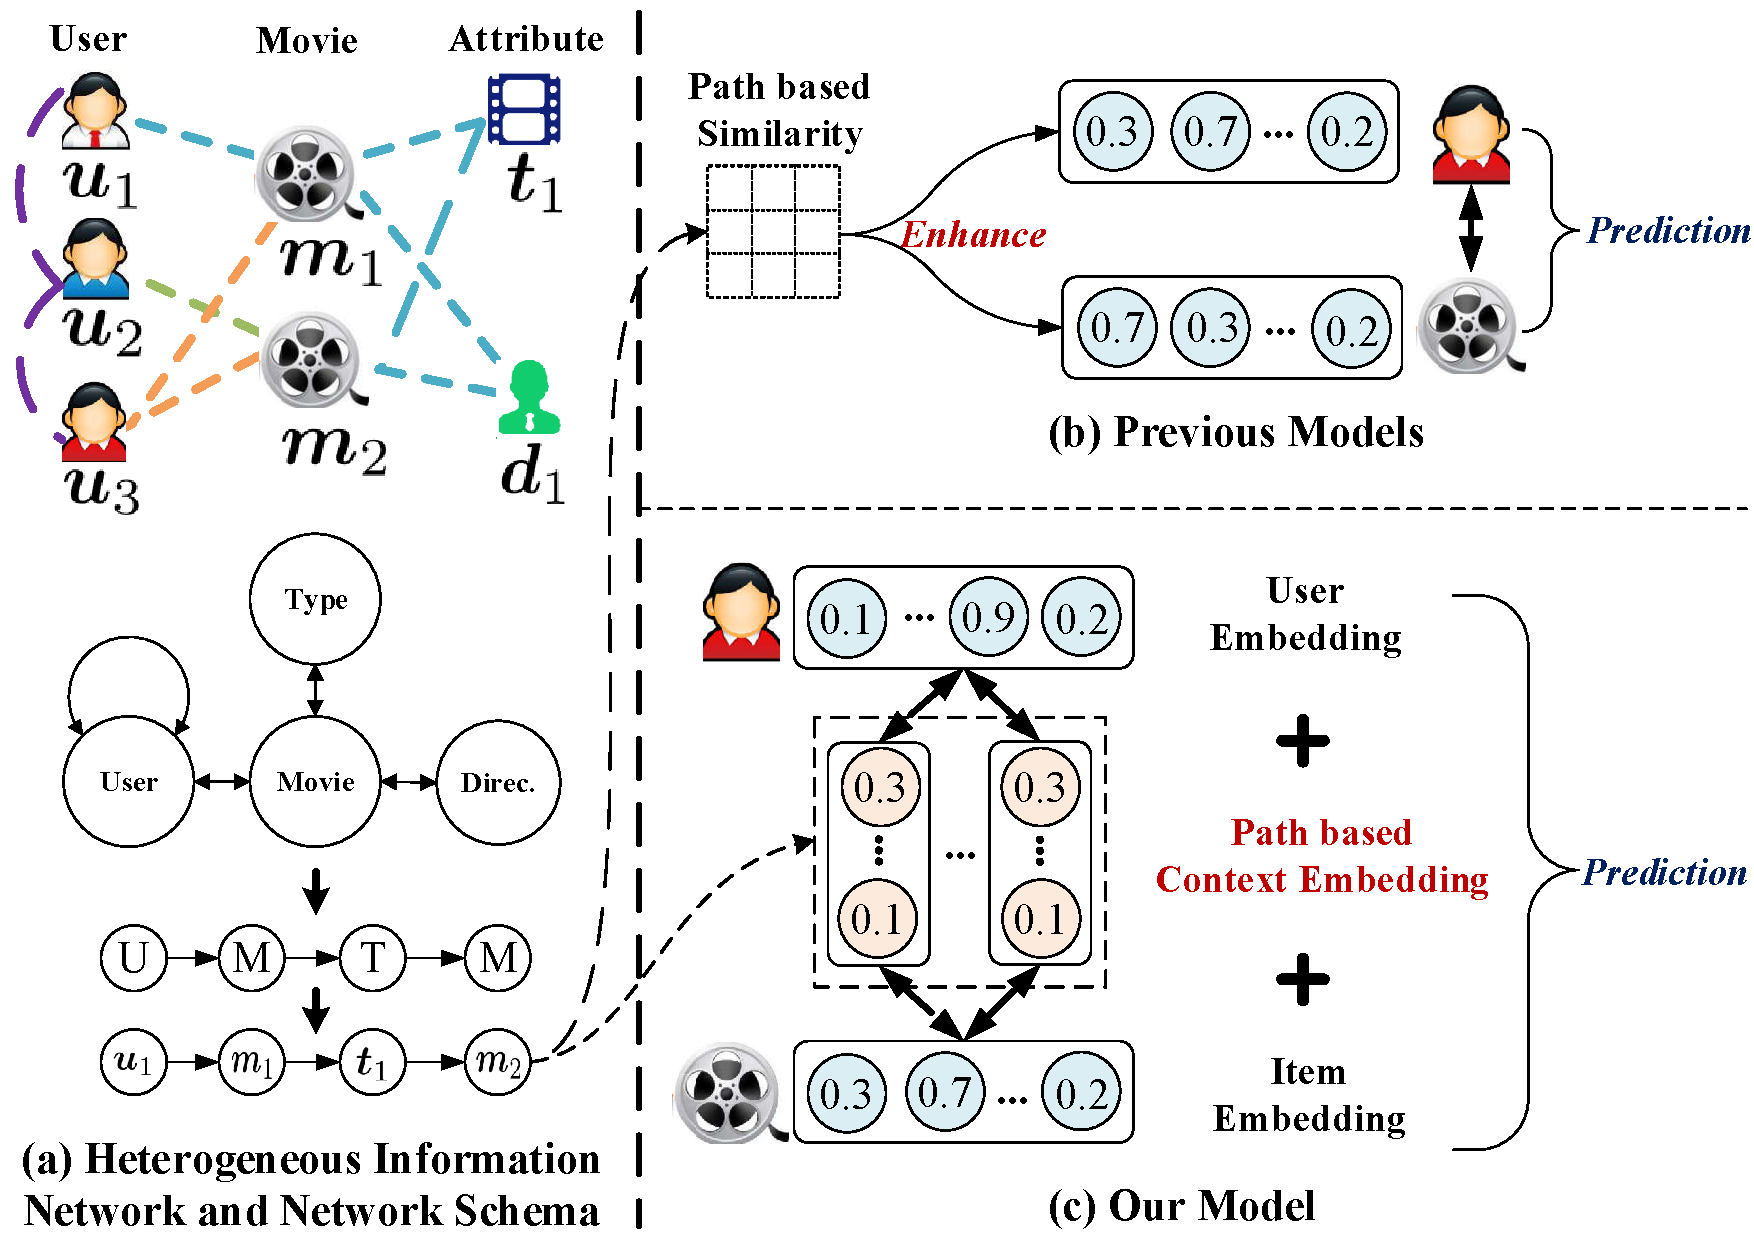
\includegraphics[width=8.5cm]{image/framework_intro.pdf}\\
  \caption{The illustration for HIN based recommendation setting (network schema, meta-path, path instance) and the comparison between our model and previous methods (two-way interaction \emph{v.s.} three-way meta-path based interaction). }\label{fig-framework-intro}
\end{figure}

To address these issues, we aim to leverage rich meta-path information from HIN for top-$N$ recommendation in a more principled way. For convenience,  given a target user-item pair, we call the aggregate meta-paths (together with their corresponding path instances) connecting the user with the item \emph{meta-path based context} of the interaction.
Our main idea is to (1) learn explicit representations for  meta-path based context tailored for the recommendation task, and (2) characterize a three-way interaction of the form:  $\langle$\emph{user}, \emph{meta-path}, \emph{item}$\rangle$. The paradigm of our work is illustrated in Fig.~\ref{fig-framework-intro}(c).
By explicitly incorporating meta-paths into the interaction model,  our approach is able to effectively mine and extract useful information from meta-path based context for improving the recommendation performance.
In this way, the characterization of  meta-path based context will be more flexible to adapt to different interaction scenarios, providing a good
interpretability on the recommendation results, \ie \emph{who} will adopt \emph{what} given the \emph{context}.
The idea is appealing, while the solution is challenging.  We have to consider three key research problems: (1) how to design the base architecture that is suitable for the complicated HIN based interaction scenarios; (2) how to generate meaningful path instances for constructing high-quality meta-path based context; and (3) how to capture the mutual effect between the involved user-item pair and meta-path based context in an interaction.

In this paper, for tackling various complicated interaction scenarios,  we adopt deep neural networks to build the base architecture for our recommender, since it has been shown that deep neural networks are more capable of learning arbitrary interaction function from data~\cite{he2017neural}.
We elaborately design a three-way neural interaction model by explicitly incorporating meta-path based context into the interaction.
 To construct the meta-path based context, we propose to use a 
 priority based sampling technique to select high-quality path instances for recommendation, since a simple meta-path guided sampling strategy like that in \cite{dong2017metapath2vec} is likely to generate low-quality path instances or even noise for our task.  Our model needs to learn the representations for users, items and meta-path based context.
We propose a novel co-attention mechanism to mutually improve the representations for  meta-path based context, users and items. Specially, the  representations for meta-path based context are first improved according to the information from a user-item pair in an interaction, and then user and item representations are further enhanced conditioned on the improved representations of meta-path based context.
 In this way,  the  meta-path based context are transformed into a form that is directly useful for a specific interaction, which is supposed to be more effective in recommendation than original representations.
Meanwhile, the improved user and item representations also embody useful evidence from calibrated meta-path based context for the current interaction.
By comparing Fig.~\ref{fig-framework-intro}(b) and (c),
we can see that, different from previous methods, our proposed model explicitly incorporates the meta-path based context into the interaction, and learns interaction-specific representations for these useful information.

%Our main idea is to learn interaction-specific representations for \emph{meta-path based context} in recommendation, and the learned  representations  are  involved as an explicit factor for modeling user-item interactions. We consider meta-paths as interaction context to bridge a user and an item, and characterize a three-way interaction of the form:  $\langle$ \emph{user}, \emph{meta-path}, \emph{item} $\rangle$.
%By explicitly learning interaction-specific meta-path representations,  the proposed approach is more adaptive and effective in modeling varying user-item interactions. In addition, by framing meta-path based information as interaction context, the approach is expected to have good model interpretability on the recommendation results, \ie \emph{who} will adopt \emph{what} given the \emph{context}.
%Since the recommendation task in HIN is usually complicated and difficult, we develop our approach based on the recent neural collaborative filtering framework~\cite{he2017neural} in implementing a powerful interaction function.
%Different from   \cite{he2017neural}, our interaction function is able to characterize three-way interaction by incorporating an explicit representation factor for the involved meta-path contexts in an interaction.
%The idea is intuitive, while the solution is challenging.  To implement the idea, we have to consider (1) how to generate useful interaction-specific path instances from some meta-path, and (2) how to make the meta-path representation adaptive to a specific  interaction.

%For the first problem, we find that using a simple meta-path guided sampling strategy like that in \cite{dong2017metapath2vec} is not effective to generate useful paths as interaction contexts.  The reason is that HIN is usually highly connected and contains many path instances for a single meta-path. Among these path instances, it is likely that only a few contain useful evidence for a single interaction.
%Based on this consideration, we pretrain a classic recommendation model with implicit feedback, \ie the Bayesian Personalized Ranking model (BPR)~\cite{rendle2009bpr},  for guiding the path generation process.  A path will be sampled only if it is consistent with the relevance evidence from the BPR model.

%borrow the \emph{pretrain} idea for training neural networks, and improve the sampling strategy by incorporating a heuristic method which are guided by both meta-paths and pretrained traditional implicit recommendation methods, \ie BPR~\cite{rendle2009bpr}.
%We force the sampling process to follow the path which is more consistent to the relevance evidence from BPR.

%For the second problem, we carefully design a hierarchical meta-path representation method. It first embeds a single path instance,  then represents a single  meta-path based on multiple  embeddings of its path instances, and finally aggregates multiple meta-path embeddings as the representation of the meta-path based context.  The most difficult point lies in how to make the representations of  meta-path based context flexibly adapt to varying interactions,  providing high-quality recommendation evidence. To solve this problem, we propose a novel co-attention mechanism to alternatively improve the representations for  meta-path based context, users and items. Specially, our  representations for meta-path based context are first improved according to the information from a user-item pair in an interaction, and then user and item representations are further enhanced according to the improved representations of meta-path based context. In this way,  the  meta-path based context are transformed into a form that is directly useful for a specific interaction, which is supposed to be more effective in recommendation than original representations. In addition, the improved user and item representations also embody useful evidence from elaborated meta-path based context.

To our knowledge, it is the first time that  meta-path based context has been explicitly modeled in a three-way neural interaction model, \ie $\langle$\emph{user}, \emph{meta-path}, \emph{item}$\rangle$, for the task of top-$N$ recommendation in HIN.
We propose a novel deep neural network with the co-attention mechanism by leveraging rich meta-path based context, which is able to learn interaction-specific representations for users, items and meta-path context.
We do extensive experiments on three real-world datasets, which demonstrate the effectiveness of the proposed model compared to the state of arts.
In addition, we also validate that the proposed model has the potential to alleviate cold-start problem and provide interpretable recommendation results.

%We construct extensive experiments on three real-world datasets demonstrate the effectiveness of the proposed model. Moreover, we show the capability of the proposed model for the cold-start prediction problem, and reveal that the impact of different meta-paths for recommendation via the proposed attention mechanism.


%For the above issues, it is challenging to develop a way to effectively extract and represent useful information for HINs due to data heterogeneity. Unlike previous studies using meta-path based similarities\cite{yu2013collaborative,zhao2017meta}, our idea is to learn effective representations between users and items for summarizing important structural characteristics and properties of HINs. Hence, we propose a new heterogeneous network embedding method to embed the relation between users and items. Considering heterogeneous characteristics and rich semantics reflected by meta-paths, we introduce a heuristic random walk guided by meta-paths to sample path instances (node sequences) between users and items. For each path instance, we learn a unique embedding representation representation for a user-item pair by convolution neural network. According to the assumption that the important feature in each embedding usually has high value, we utilize the max pooling layer to fuse the multiple embeddings \wrt different path instances as the output of CNN.

%After obtaining the user embeddings, item embeddings and the relation representation between users and items, we study how to integrate and utilize such information for top-$N$ recommendation. Traditional recommendation methods usually only consider the interaction between users and items, and utilize simple multiplication to uncover this complex interaction. Instead, we propose and explore the interaction between users, items and the user-item pairs and apply deep model (MLP) to model their interaction in order to endow the model a large level of flexibility and non-linearity for recommendation. For the interaction between users, items and user-item pairs, we proposed a novel neural attention mechanism for the fusion of path embedding under different meta-paths and the adjustments of user and item embeddings, respectively.
%
%By integrating the above description together, this work presents a novel meta-path based recommendation model. The proposed model first extract user-item pair's embedding according to meta-path in the HIN and encode users and items as well. And then we utilize neural attention mechanism to characterize the interaction of users and items for the top-$N$ recommendation. Extensive experiments on three real-world datasets demonstrate the effectiveness of the proposed model. We also verify the ability of the proposed mode to alleviate cold-start problem and examine the impact of meta-paths on performance. The key contributions of this paper can be summarized as follows:

%\textbullet\ We proposed a novel deep model for top-$N$ recommendation based on heterogeneous information networks to leverage rich information and semantics in RS. To our best knowledge, it is the first attempt to exploit structure information in HIN with the neural network for top-$N$ recommendation.

%\textbullet\ The proposed HeteRank model designs a deep neural network to learn the embedding of node pair, which is seldom studied in previous HIN embedding. Different from widely used path based random walk strategy in HIN embedding, we design a similarity guided  random walk strategy based on meta path, which can effectively capture structure features with less time cost.

%\textbullet\ We firstly propose a cooperative attention mechanism to fuse different embeddings for recommendations.  The cooperative attention mechanism utilizes the embedding of users and item for the better pair embedding, and leverages the pair embedding to make the embedding of users and items more suitable for recommendation.

%\textbullet\ Extensive experiments on three real-world datasets demonstrate the effectiveness of the proposed model. Moreover, we show the capability of the proposed model for the cold-start prediction problem, and reveal that the impact of different meta-paths for recommendation via the proposed attention mechanism.

